\chapter{Results}


This section describes the results of refactoring pyProCT with pyCOMPSs. It is divided into three subsections. The first one reports the benefits of using pyCOMPSs programming model. The second subsection contains the performance analysis of the results. Finally, the last part deals with tools that the framework offers.

\section{Tools}

COMPSs tools offers a great way to inspect the code executions as well as the resource usage and parallelization technique. Figure \ref{par:graph} shows an example of the tasks graph generated by pyProCT. 

This execution was limited to four algorithms (blue) and two analysis (yellow) tasks to keep it simple. We can observer that all blue tasks are executed on parallel because they have no dependencies. Red octagons are the synchronization points. Their descending structure is due to how pyCOMPSs deals internally with lists of future objects but they all belong to the same wait loop. After the clustering tasks and results retrieval (dependencies d8), the analysis tasks have the required data to be executed (d12): the generated clusterings. After them no more tasks are left and the execution is resumed (7).

Thanks to this tool we can assure that theoretical planning is correct and optimal: the graph clearly shows that the execution is embarrassingly parallel. The monitor generates the graph on-the-fly so the user can check the application work flow while it is running helping to identify bottlenecks and other execution-time issues.

\begin{figure}[h]
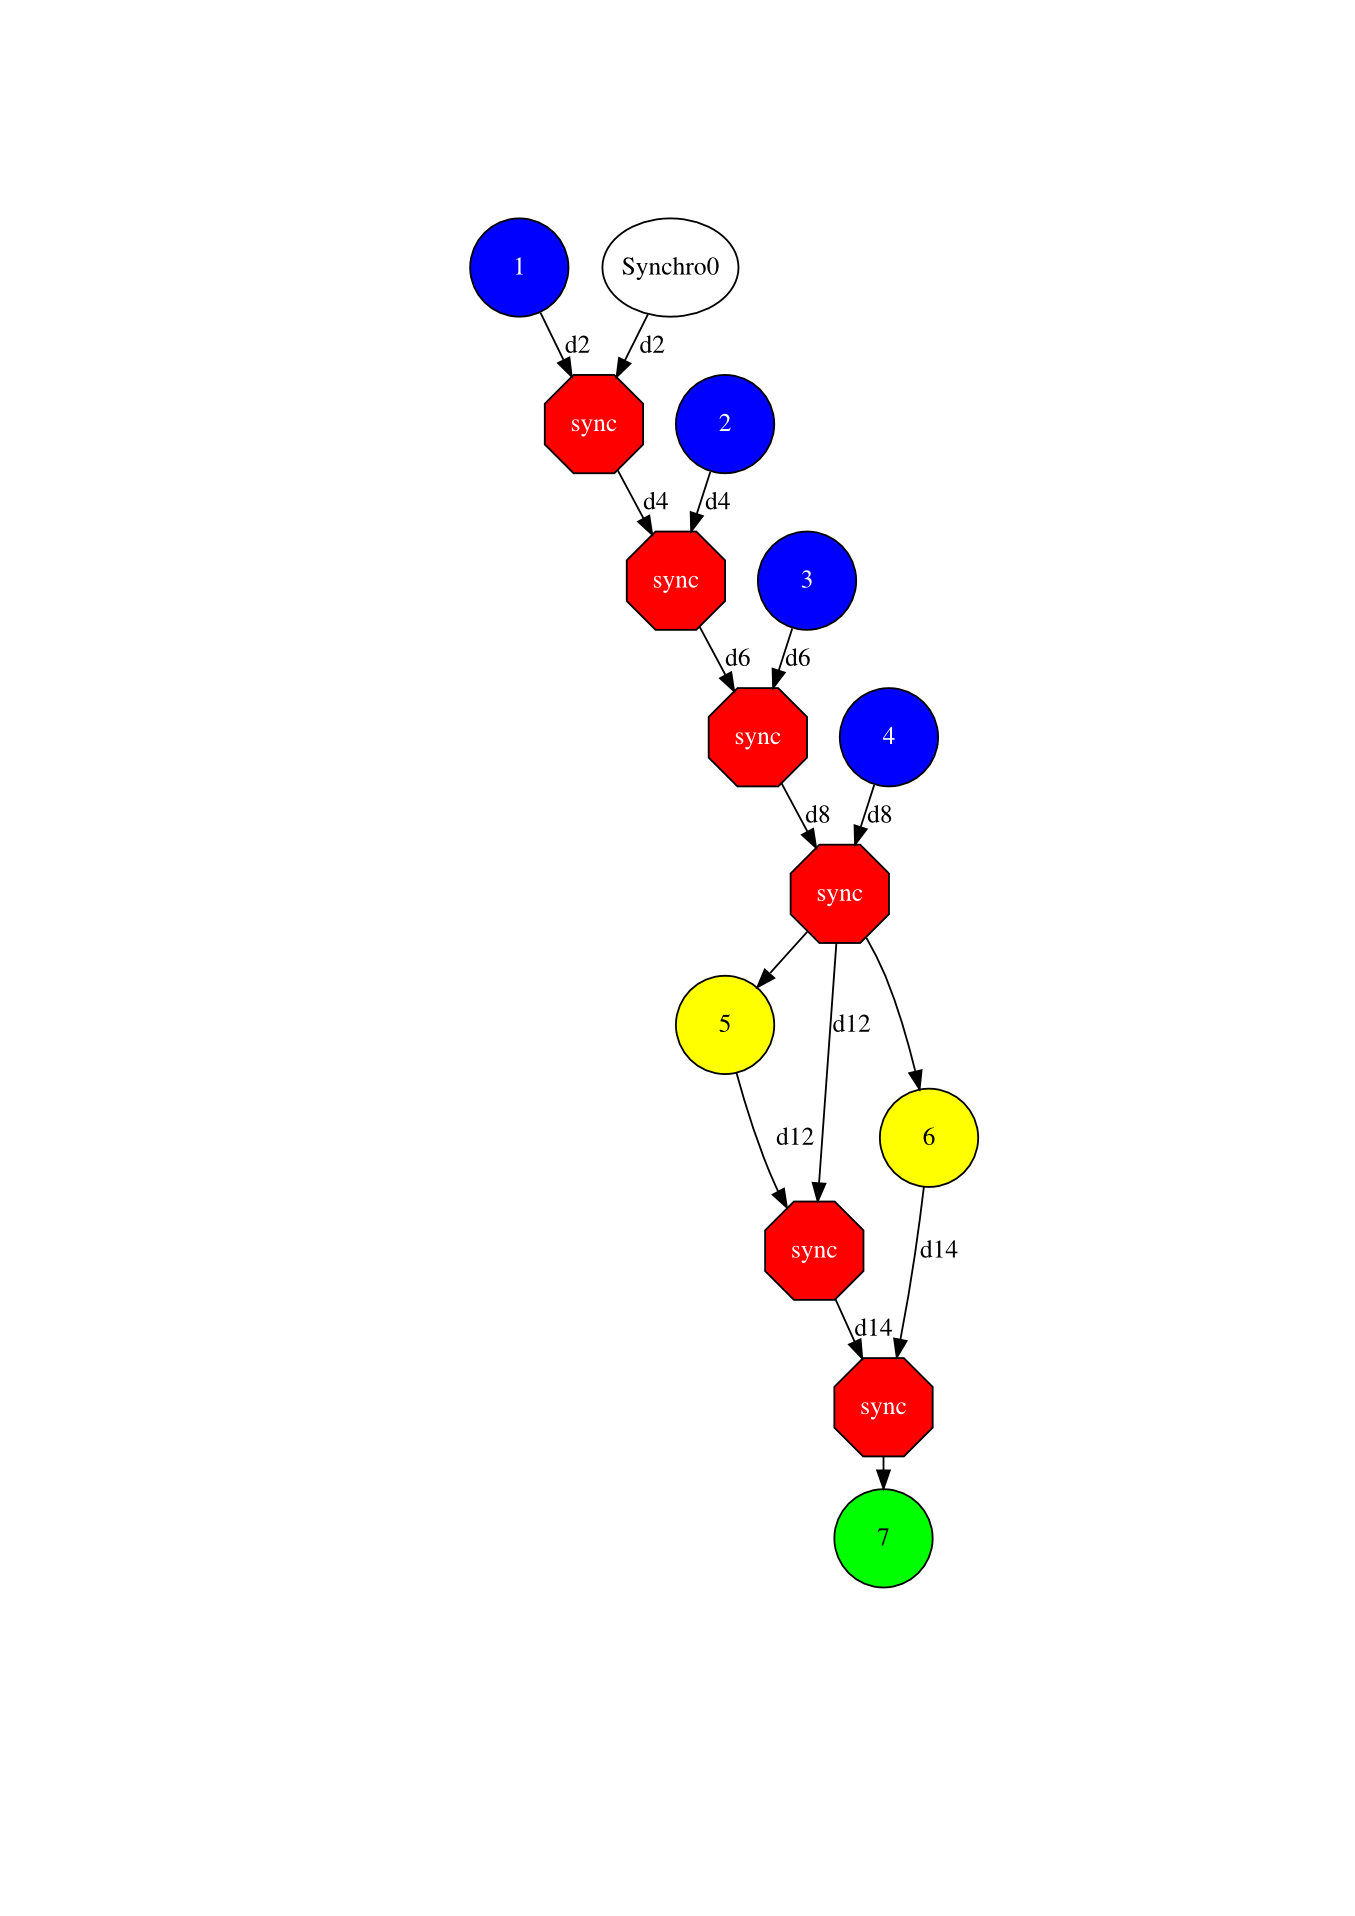
\includegraphics[height=\textheight]{img/main_01_completeGraph.png}
\caption{COMPSs monitor graph for 4 threads and small dataset}
\label{par:graph}
\end{figure}

The monitor also offers an execution and tasks information tab. There, for each task type, we can check which is its jobs IDs (in order to identify it on the traces), the host where it was executed, the job status, the number of execution and its average time. 

Figure \ref{fig:monitor} shows the information associated to the previous execution graph. We see that the most expensive computation are the clustering ones. Not only their execution time is almost twice the analysis' one but the executed count is also the double.

 \begin{figure}[h]
 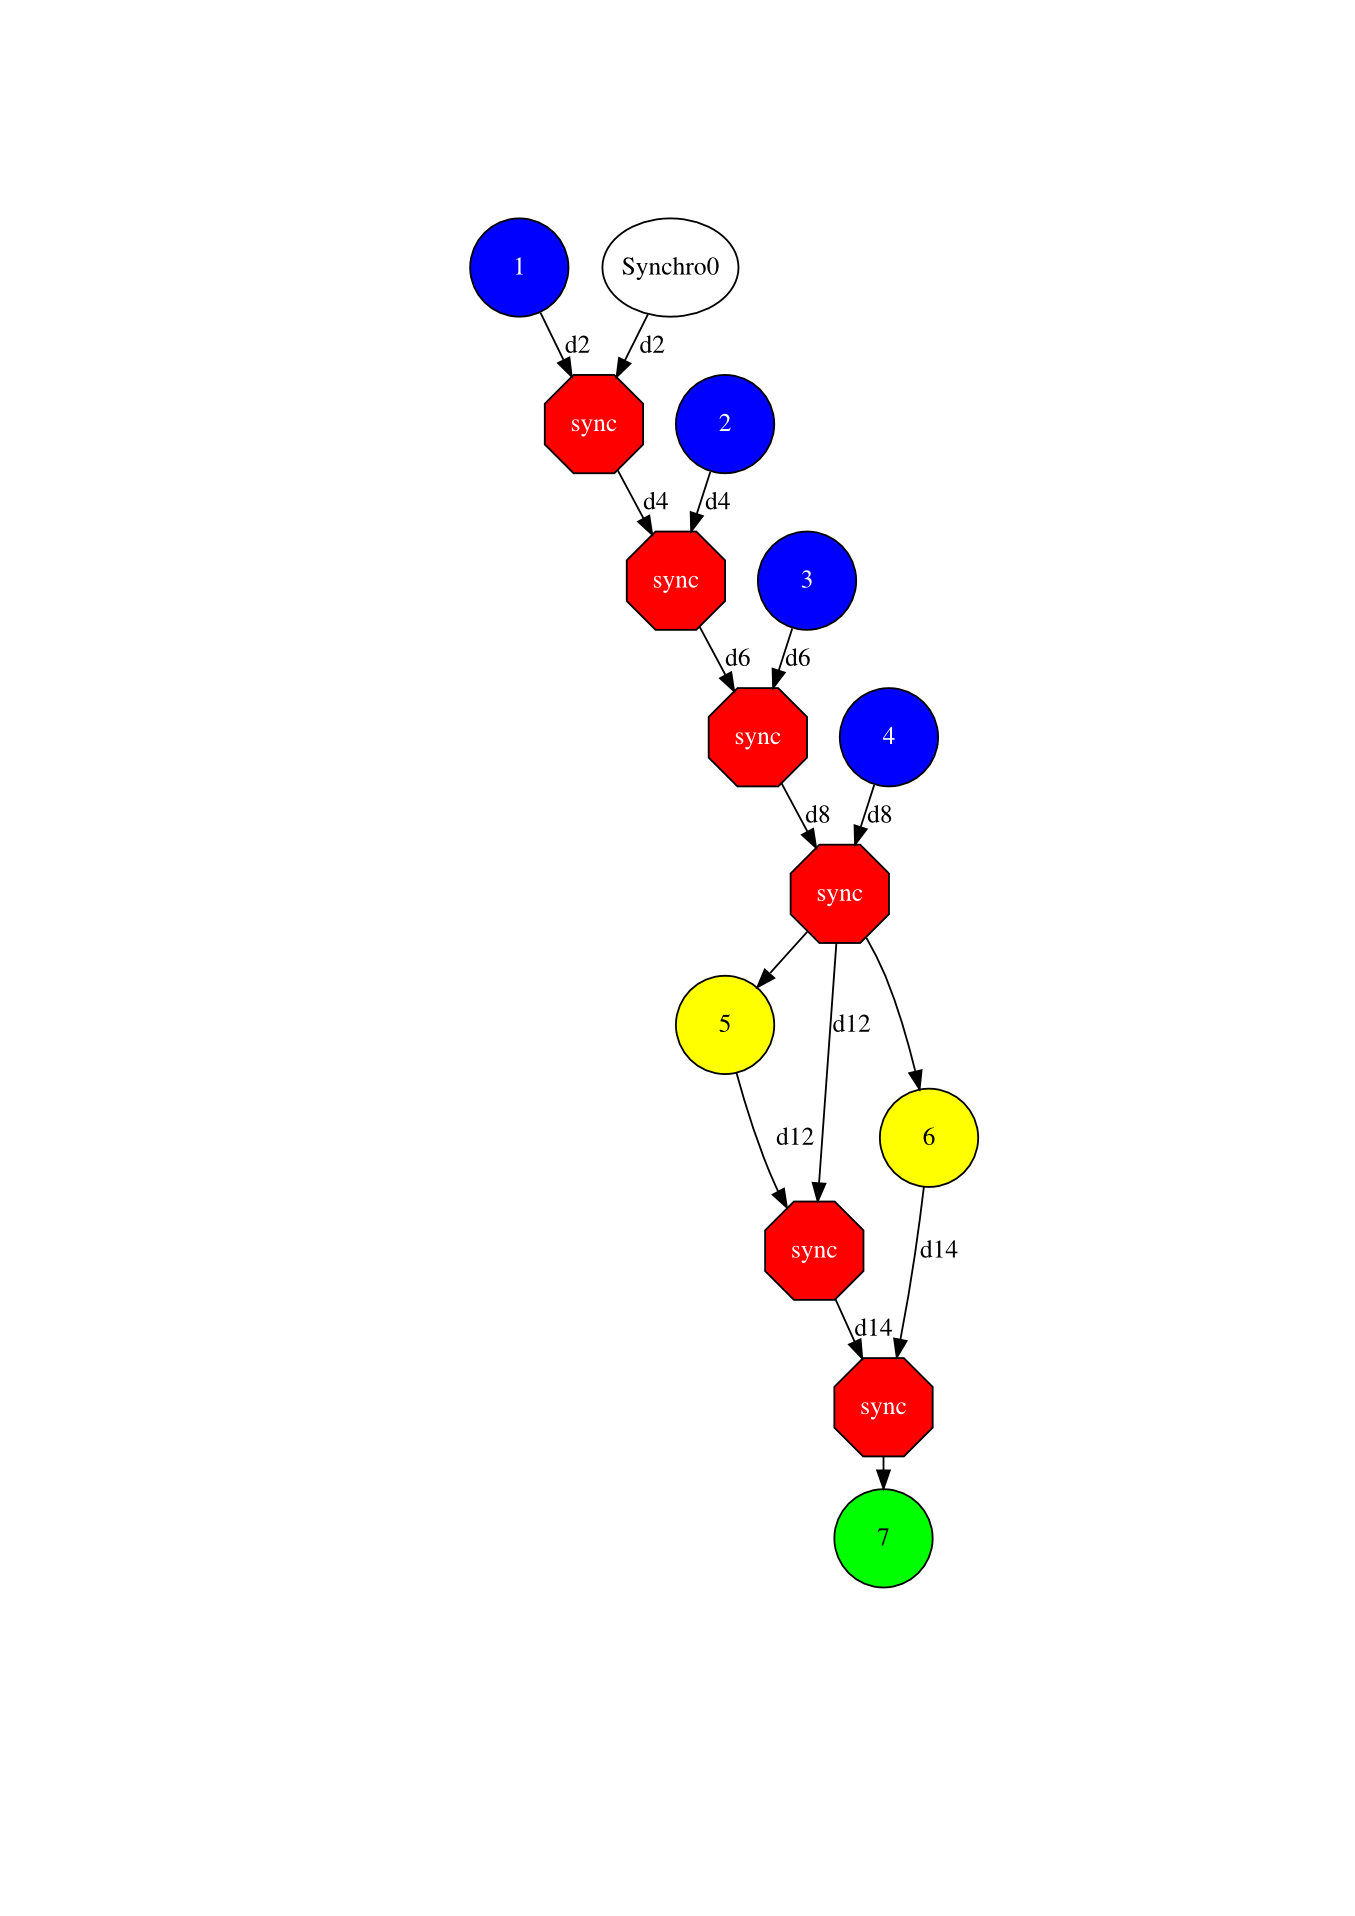
\includegraphics[height=\textheight]{img/main_01_completeGraph.png}
 \caption{COMPSs monitor tasks information}
 \label{fig:monitor}
 \end{figure}
 
 
 The tracing system has also been an invaluable asset. It allows to generate traces just by setting a flag on the execution. On the other hand, for MPI and parallel a lot of time was spent in order to get traces. Next results' section \ref{sec:resperformance} shows plenty of them and how they were key to some of the optimizations performed.

\section{Programming Model}

PyCOMPSs framework is supposed to require little extra code to be used so first a comparison between the difference of size of each version will be made. Figure \ref{tab:sizes} shows the comparison between the different classes required. It is based on the number of characters and lines because python conventions encourage the usage of line breaks so the results could be misleading (some functions have one parameter per line).


\begin{center}
	\begin{tabular}{| R{6cm} | L{3cm} | L{3cm} |}
		\hline
		Class Name & Original & pyCOMPSs \\ 
		\hline
		\hline
		Driver & 169 / 8180  &  165 / 7911 \\
		\hline
		ClusteringProtocol & 78 / 3703 & 73 / 3490 \\
		\hline
		PostProcessingDriver & 32 / 1531 & 56 / 2700 \\
		\hline
		ClusteringExplorer & 195 / 8470 & 197 / 9226 \\ 
		\hline
	\end{tabular}
	\captionof{table}{Size comparison of duplicated classes} 
	\label{tab:sizes}
\end{center}


We see that the refactor did not add too much space. The driver and protocol classes are in fact shorter. This is caused because of the removal of the task-adding loop and the pyScheduler initialization. Postprocessing driver is longer due to the fact that on the original version this section is not parallel. The other ones are quite even.

PyCOMPSs framework just uses python decorators and API calls so, why do we observe a size increase in some classes? This is due to the fact that our data can not automatically serialized by python's pickle. Almost all the extra size is linked to the work needed to handle the matrix data. However, other than adding this little size overhead, the code is much clean and easy to read. 

Another important aspect is the execution process and tools offered by the framework. It is here were COMPSs truly shines. 

The level of hardware abstraction provided by the framework is really good. To execute pyProCT in a local environment one just needs to provide the language (python on this case), classpath, executable and parameters. If the user desires to customize the framework offers two kind of hardware configurations. On the one hand we find the \textit{resources.xml}. This file allows to define the workers to be used. This includes supercomputer nodes, cloud services, remote images and more. On the other hand we have the \textit{project.xml} which selects which of the defined resources are to be actually used and some runtime parameters. 

With this simple two files we can define a wide range of available resources to be used and then select which ones we want to use for an specific execution. Thanks to this we can use a lot of different resources without worrying about the internals and communications. COMPSs' already implements all the connectors required to use them so we just need to give a description of them, select which to use and decorate our code. 

For MareNostrum III executions this process is even easier. The development team has created scripts to submit jobs to the supercomputer. By default, it requires the same parameters as a normal execution. However, it has a wide range of easy-to-use options with a clear description. With all the parameters available, such as the network and file system to be used or the number of nodes, it automatically creates the \textit{resources.xml} and \textit{project.xml} that best suit our needs. 

This is tools are really useful. Most of the time working of this project has been spent on trying to execute the program on the supercomputer. One needs to understand how a submission queue system works, which parameters need to be specified, how the class paths are read and used, which way the supercomputer access files, which kind of problems may arise from mutex access to the datasets and so on. This is a quite daunting task for someone without advanced knowledge on the subject or with no one to ask help to. 

As stated, COMPSs required number of parameters are far less. Understanding some of the aforementioned things will help the user to better use the framework but they are not really mandatory because the COMPSs manuals are good and clear. Following the examples is enough to execute your own programs. 



\section{Performance}

\label{sec:resperformance}

This section reports the results of the refactor related with the performance. 

Throughout this section some traces will be presented to describe the numerical results. However, the times reported on the traces can not be compared. This is due to the fact that each parallelization is instrumented with a different method (see Appendix \ref{sec:instrumentation}). Because of that we can not trust the reported times; pyCOMPSs and multiprocessing instrumentation are far slower than the MPI version because they need to create a process to emit each of the events.

When reporting execution times the x-axis will frequently contain number of threads/processes used. However, when queueing pyCOMPSs executions we specify the desired amount of nodes being the minimum 2 (one is used for the runtime/master which handles all the framework). For this reason, the executions will start at 32 processes/threads which corresponds to that 2 nodes (each node uses 16 threads). Instead, for multiprocessing the execution will be limited to 16 because it can not run on more than one node.


Table \ref{fig:datasets} shows the datasets used on the analysis:

\begin{center}
	\begin{tabular}{| C{1cm} | R{6cm} | L{3cm} | L{2cm} | L{3cm} |}
	\hline
	ID & Type & Size (Mb) & Format \\ 
	\hline \hline
	1 & Protein ensemble & 78 Mb & PDB \\
	\hline
	2 & Pprotein ensemble & 675 Mb & PDB \\
	\hline
	3 & Protein ensemble & 4.3 Gb & PDB \\
	\hline
	4 & Numeric array & 72 Kb & TXT \\
	\hline
	5 & Numeric array & 142 Kb & TXT \\
	\hline		
	\end{tabular}
	\captionof{table}{Datasets used for performance analysis}
	\label{fig:datasets}
\end{center}


\section{Scheduling order}
\label{sec:sch_oder}

This first section describes the improvement achieved by ordering the execution of the algorithms.

Figure \ref{fig:small_trace_noorder} and \ref{fig:small_trace_order} show the differences of scheduling the hierarchical and spectral algorithms first or last. On violet we have the clustering tasks and the analysis ones are on yellow. We can see that the initialization of the hierarchical and spectral is performed while the workers are executing the other algorithms. The bright red stripes on the master thread (1.1.1) correspond to the action of queueing a task. On the first one the time between the start and the stripes is the hierarchical initialization. The time between that stripes and first task is the transfer of data. Threads remain idle during that time. On the second example once queued the transfer starts so while performing the costly initialization pyCOMPSs is already transferring the data for the tasks.

From here onwards the version with the ordered execution will be always used.


\begin{figure}[h]
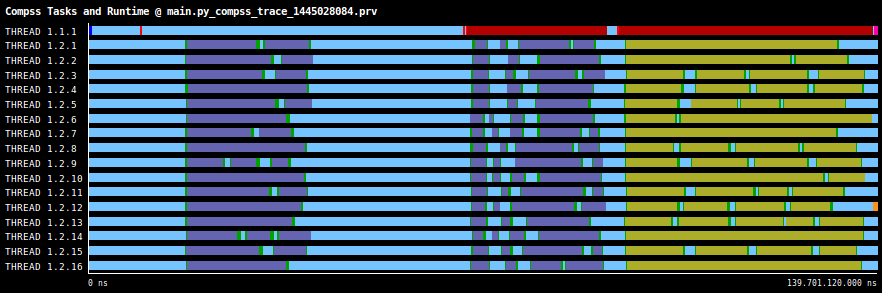
\includegraphics[width=\textwidth]{traces/compss_2_small_noorder.png}
\caption{Trace for dataset 5 without ordering algorithm's execution}
\label{fig:small_trace_noorder}
\end{figure}

\begin{figure}[h]
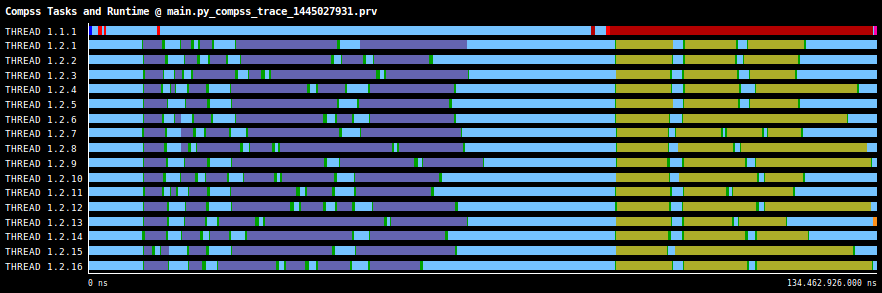
\includegraphics[width=\textwidth]{traces/compss_2_small_order.png}
\caption{Trace for dataset 5 ordering algorithm's execution}
\label{fig:small_trace_order}
\end{figure}

Next we will see an in-depth analysis of a trace for each version in order to understand the results on bigger datasets.

Figure \ref{tra:par16small} shows the trace for multiprocessing execution with 16 threads. The code is intrumented following pyProCT structure: initialization and parameters handling, data, clustering and postprocess. First blue stripe is the time from the start till the data section. The white one is the matrix handling and calculation. After that all the red section is the actual clustering and analysis. Last strip of first thread is the postprocess. The purple sections correspond to the algorithms and analysis tasks. Note that for multiprocessing the first thread also performs task but they are not shown because we preferred to mark the clustering section. Note that execution is sequential until the program reaches the clustering section where it uses the parallel scheduler. We can also observer that all tasks are equally distributed amongst all the available threads. 

\begin{figure}[h]
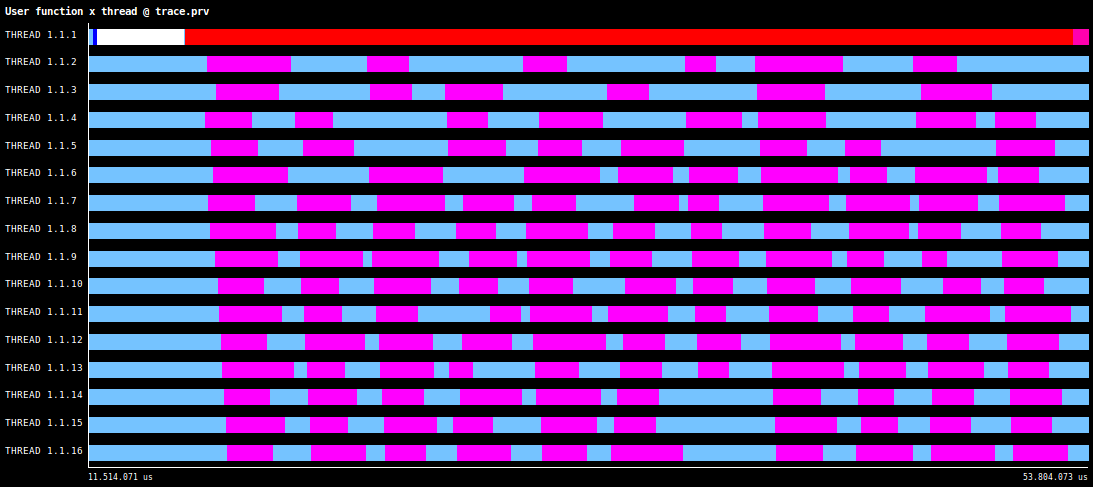
\includegraphics[width=\textwidth]{traces/par_16_small.png}
\caption{Multiprocessing scheduler with dataset 1 and 16 threads}
\label{tra:par16small}
\end{figure}

Next, figure \ref{tra:mpi16small} shows the same execution but with the MPI scheduler. First is important to see that the all the data section (in purple) and thus the matrix calculation is performed on all the threads. MPI scheduler handles the available pool of threads just when they reach the actual scheduler. That means that all the threads are doing the same work till that point and so it's redundant work. Despite that, the postprocessing section (in red) does take into the available pool and uses just one thread to avoid work duplication. 

White section is the clustering section. Inside, the green parts are the ones adding the tasks to the scheduler and the blues the actual algorithms execution. The blue stripes outside the white part are the ones corresponding to the analysis tasks (which have the same name and thus the same color).Even if all the threads are performing the task-adding loop they are added only once because the task's name must be unique. Please note that blue stripes are composed of a lot of littler ones (the number of tasks is the same on both executions)  

We can see that on MPI the matrix calculation is quite longer than the multiprocessing (with respect to its own total time as we can not compare across traces). This is because having 16 threads busy makes them all go slower because, being in the same node, they share some resources (like cache) and all of them are accessing the same input file. On the loop that adds the tasks we see again the same behaviour: duplicated work that wastes resources and increases execution time. Multiprocessing is almost all the time in parallel mode and that the sequential parts are small. MPI, on the other hand, despite running in parallel almost all the time it just does useful work in the blue stripes. However, multiprocessing is limited to 16 threads so this is it's performance peak and MPI can use more resources.

\begin{figure}[h]
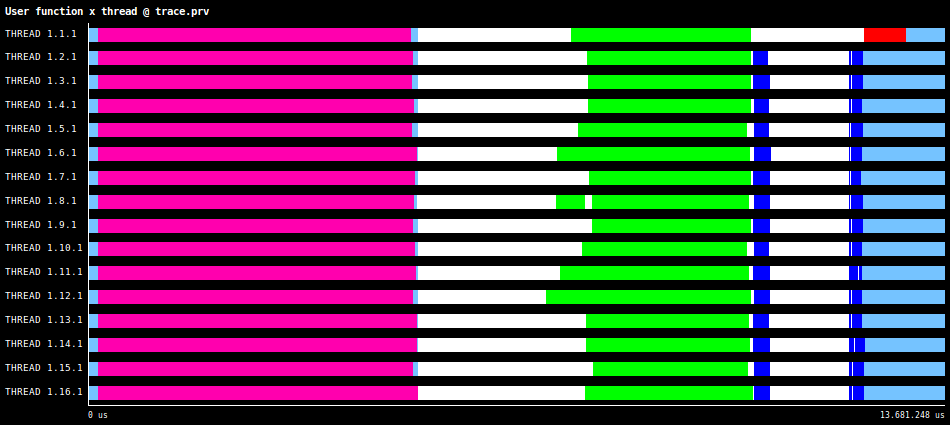
\includegraphics[width=\textwidth]{traces/mpi_16_small.png}
\caption{MPI scheduler with dataset 1 and 16 threads}
\label{tra:mpi16small}
\end{figure}

Figure \ref{fig:small_trace_order} shows the resulting trace of executing the dataset 5 with the pyCOMPSs refactor.  Even if it is not the same dataset on the other traces, for comparison purposes this is not an issue as we are just observing how tasks are distributed not comparing the actual execution times.  We see that pyCOMPSs version is almost all the time computing tasks in a embarrassingly parallel mode. 

The dark red section is the time in which the main execution is waiting for the tasks results. During the clustering section the main is always running as opposed to figure \ref{fig:small_trace_noorder} in which the main is locked during the last tasks. On the analysis part the loop that calls the tasks is fast so, once performed, the main waits for the clustering scoring results in order to choose the best and start the postprocessing.


Figure \ref{fig:small} shows that COMPSs is the slowest parallelization for the dataset 1 and the multiprocessing is the fastest. That is caused because this method is only able to work on a single node so the initialization and overhead of data and resources handling is indeed much smaller. For this first example we have used the best result found for each version, that is: 16 threads for multiprocessing, 12 threads for MPI and 2 nodes for pyCOMPSs.

 Figure \ref{fig:graph} shows the executions times (normalized to 1) of the three versions for dataset 1, 2, 3 and 4. MPI and multiprocessing crash with dataset 3 if we use too much threads. That causes the performance reduction for multiprocessing on datset 3 because it only is able to run with maximum 8 threads. We observe that for  datasets 3 and 4, which are the most demanding, COMPSs outperforms MPI a lot and improves multiprocessing. Table \ref{fig:times} shows the actual numerical results.


\begin{figure}[h]
\centering
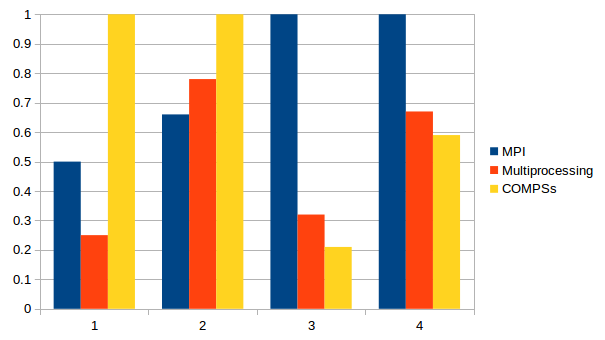
\includegraphics[scale=0.85]{img/graph.png}
\caption{Relative execution times for three versions and datasets 1, 2, 3 and 4}
\label{fig:graph}
\end{figure}

\begin{center}
	\begin{tabular}{| C{3cm} | C{3cm} | C{3cm} | C{3cm} | C{3cm} |}
	\hline
	Version & Dataset 1 & Dataset 2 & Dataset 3 & Dataset 4 \\ 
	\hline \hline
	COMPSs & 24 s & 88 s & 660 s & 1473 s \\
	\hline
	MPI & 12 s & 58 s & 3100 s & 2483 s \\
	\hline
	Multiprocessing & 6 s & 74 s & 992 s & 1670 s \\
	\hline
	\end{tabular}
	\captionof{table}{Execution times of three versions}
	\label{fig:times}
\end{center}



Table \ref{fig:small_times_tab} shows the execution times for dataset 1 given by the number of threads. Multiprocessing can use a maximum of 16 threads and COMPSs requires at least 32 so the other boxes are empty for them. We see that the dataset is too small to benefit from the parallelization because adding resources does not improve the performance. Clearly multiprocessing is the best. MPI's performance decreases with the number of threads, this is probably caused by the replication of work on all the threads.



\begin{center}
	\begin{tabular}{| C{3cm} | C{2cm} | C{2cm} | C{2cm} | C{2cm} |  C{2cm} | C{2cm} |}
	\hline
	Version & 4 & 8 & 16 & 32 & 48 & 64 \\ 
	\hline \hline
	COMPSs & - & - & - & 24.3 s & 23.2 s & 24.4 s\\
	\hline 
	MPI & 9.6 s & 10.2 s & 12.1 s & 13.02 s  & 13.2 s & 14.4 \\
	\hline
	Multiprocessing & 6.1 s & 6.0 s & 6.1 s & - & - & - \\
	\hline
	\end{tabular}
	\captionof{table}{Execution times of dataset 1 given by number of threads}
	\label{fig:small_times_tab}
\end{center}


Dataset 2 execution times can be seen on table \ref{fig:medium_times_tab}. Here COMPSs already outperforms both other methods. Still, pyProCT is not escalating with the resources for the refactored code. On MPI we see that we reach the best performance at 
32 threads. Multiprocessing escalates really well but can not use more than 16 threads.
\begin{center}
	\begin{tabular}{| C{3cm} | C{2cm} | C{2cm} | C{2cm} | C{2cm} |  C{2cm} | C{2cm} |}
	\hline
	Version & 4 & 8 & 16 & 32 & 48 & 64 \\ 
	\hline \hline
	COMPSs & - & - & - & 58.9 s & 57.3 s & 59.1 s\\
	\hline 
	MPI & 144.2 s & 97.6 s & 86.4 s & 80.6  & 85.3 s & 89.3 \\
	\hline
	Multiprocessing & 133.2 s & 105.6 s & 67.1 s & -  & -  & - \\
	\hline
	\end{tabular}
	\captionof{table}{Execution times of dataset 2 given by number of threads}
	\label{fig:medium_times_tab}
\end{center}

Dataset 3 is the biggest protein ensemble dataset and its results are reported on Table \ref{fig:big_times_tab}. The new empty boxes on MPI and multiprocessing represent the inability of the program to finish correctly. The size of the matrix is probably the cause of the crashes. Spectral algorithm also computes another matrix adding more memory load. In MPI having the aforementioned work replication the matrix rapidly grows consuming all the available memory and thus crashing. In multiprocessing the effect is the same although not having that duplication allows it to work well till 8 threads. On the other hand, COMPSs runs on multiple nodes and has more available. Also the computed matrix and the custom matrices required by some algorithms are not on the same node.

\begin{center}
	\begin{tabular}{| C{3cm} | C{2cm} | C{2cm} | C{2cm} | C{2cm} |  C{2cm} | C{2cm} |}
	\hline
	Version & 4 & 8 & 16 & 32 & 48 & 64 \\ 
	\hline \hline
	COMPSs & - & - & - & 667.2 s & 688.3 s & 687.9 s\\
	\hline 
	MPI & 3801.6 s & - & - & -  & - & - \\
	\hline
	Multiprocessing & 1447.1 s & 992.6 s & - & -  & -  & - \\
	\hline
	\end{tabular}
	\captionof{table}{Execution times of dataset 3 given by number of threads}
	\label{fig:big_times_tab}
\end{center}

Last results are the ones from the numerical dataset 4 reported on table \ref{fig:m_times_tab}. Again, some of the MPI and multiprocessing crashed. We can observe the same traits that we have been seeing during all the analysis. MPI is the slowest on large datasets and crashes on more than 16 threads rendering useless its ability to run over different nodes on distributed systems as MareNostrum 3. Multiprocessing again escalates really well till its limit. COMPSs outperforms both on big datasets and does not crash due to its ability to distribute memory load over different nodes. However we have also seen that COMPSs execution times do not benefit from the resources' increase. Next we will have a look at why that happens.
\begin{center}
	\begin{tabular}{| C{3cm} | C{2cm} | C{2cm} | C{2cm} | C{2cm} |  C{2cm} | C{2cm} |}
	\hline
	Version & 4 & 8 & 16 & 32 & 48 & 64 \\ 
	\hline \hline
	COMPSs & - & - & - & 1603.2 s & 1506.3 s & 1473.2 s\\
	\hline 
	MPI & 2581.1 s & 2543.9   & 2483.7 s & -  & - & - \\
	\hline
	Multiprocessing & 2500.1 s & 1858.6 s & 1689.0 s & -  & -  & - \\
	\hline
	\end{tabular}
	\captionof{table}{Execution times of dataset 3 given by number of threads}
	\label{fig:m_times_tab}
\end{center}


Figure \ref{fig:scalability} shows why COMPSs execution times do not decrease with the resouces' increase. Both figures show the section corresponding to the algorithm's execution of a trace. The upper ones uses 6 nodes and the lower 2. The time scale is the same on both. Green flags mark the start of each tasks (because being so close one would not be able to see it). We see that the problem is that the longer algorithms are the bottleneck of the clustering section. For two nodes, they shadow the execution time of all the smaller algorithms. When executing it on six nodes all small tasks are executed in an embarrassingly parallel fashion. However, the time is not decreased as the execution is locked waiting for the most time-consuming ones.

\begin{figure}[h]
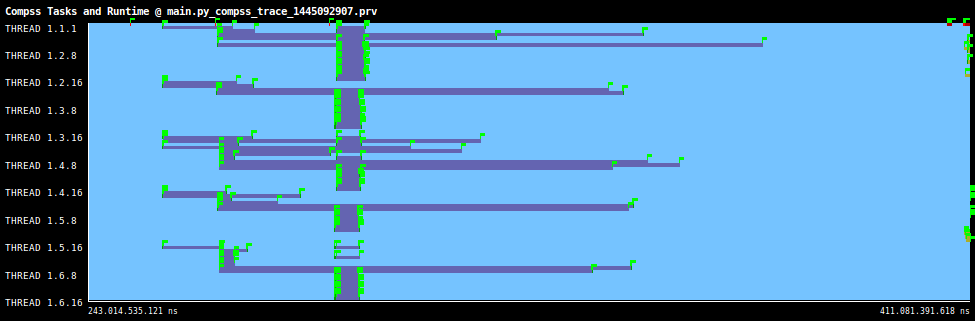
\includegraphics[width=\textwidth]{traces/compss_6_piece_tasks.png}
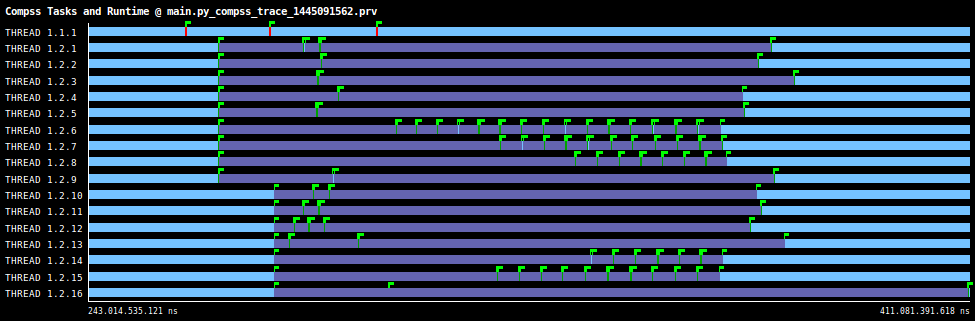
\includegraphics[width=\textwidth]{traces/compss_2_piece_tasks.png}
\caption{Section of traces for execution of dataset 4 with 6 nodes (upper) and 2 nodes (lower)}
\label{fig:scalability}
\end{figure}




 